% !TeX spellcheck = en_US
% !TeX encoding = UTF-8
% !TeX root = ../document.tex

\chapter{Running on a Validation Sample}
After the entire optimization has been performed on the \sumpT distribution of exclusive event classes, the validations must run on a separate subset of data. There are two options: the analysis of inclusive event classes or scanning of a different distribution. The latter option is favored and chosen because it keeps the number of event classes approximately the same. Thus, the validation run is performed on the \Minv distribution. As proposed in the previous chapter, the Quickscan number of candidate regions is fixed to $\paramregions = \num{200}$. 

The other settings for the validation run can be found in table \ref{tbl:music_configuration}. This configuration does not allow for a deterministic run, thus some random deviation of \ptilde is expected. When comparing the result of the Quickscan run with a full scan, the random deviation of \ptilde will show up as a finite width of the \sigmarel distribution. This width is then compared to a \sigmarel distribution obtained by comparing the results of two full scans.

\begin{figure}
	\centering
	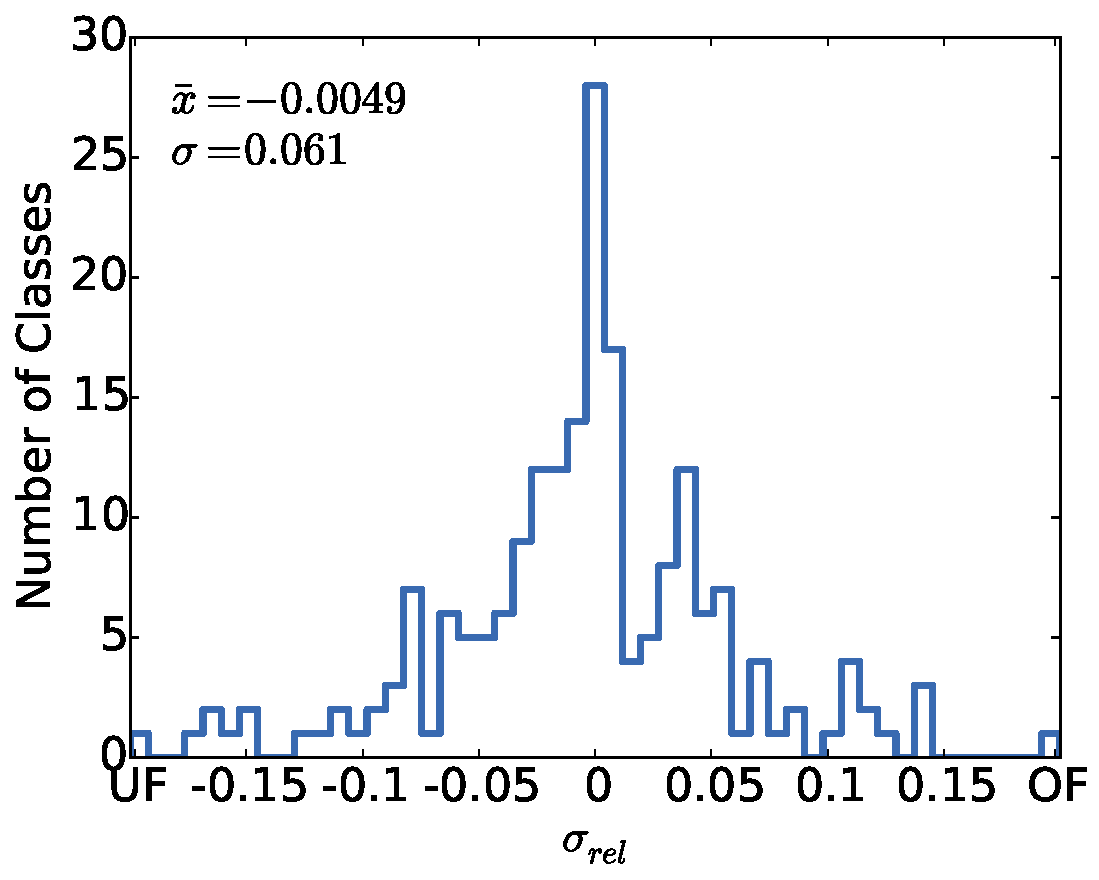
\includegraphics[width=0.49\linewidth]{delta_p_tilde_validation_random_deviation} \\
	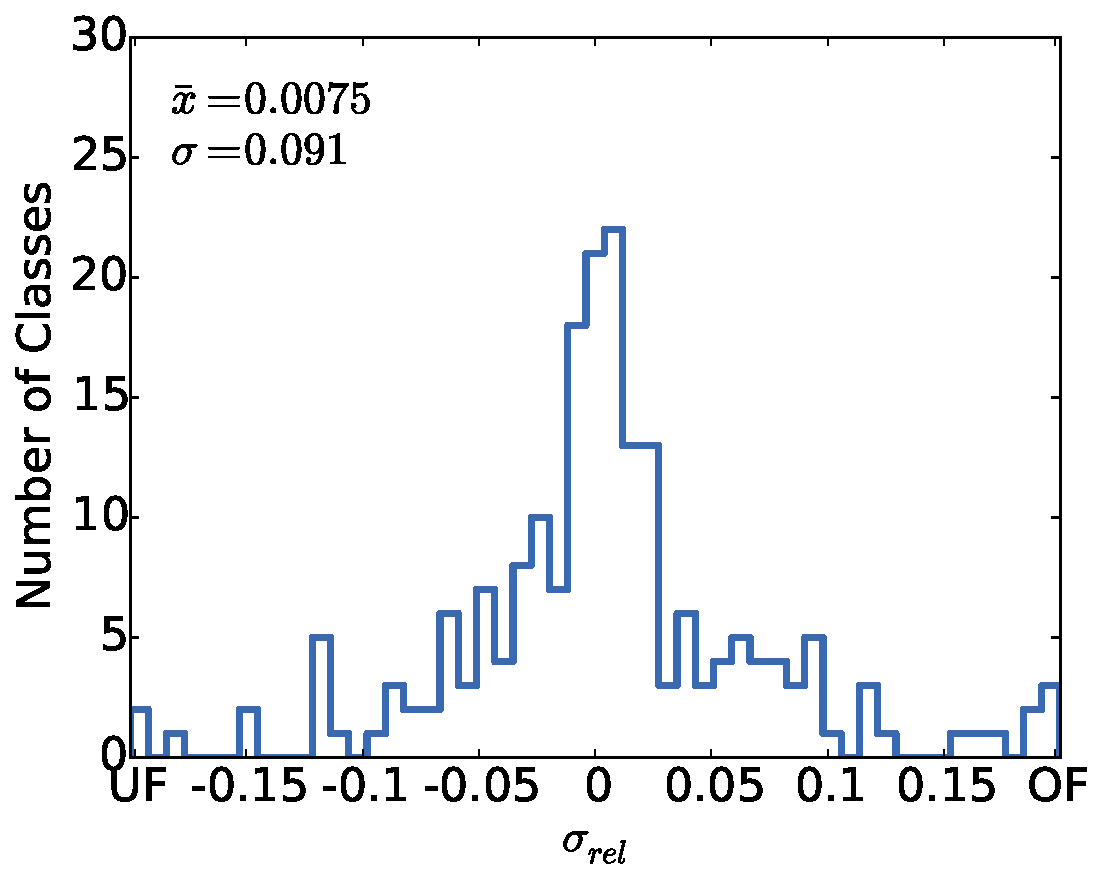
\includegraphics[width=0.49\textwidth]{delta_p_tilde_validation_f1vqs1}		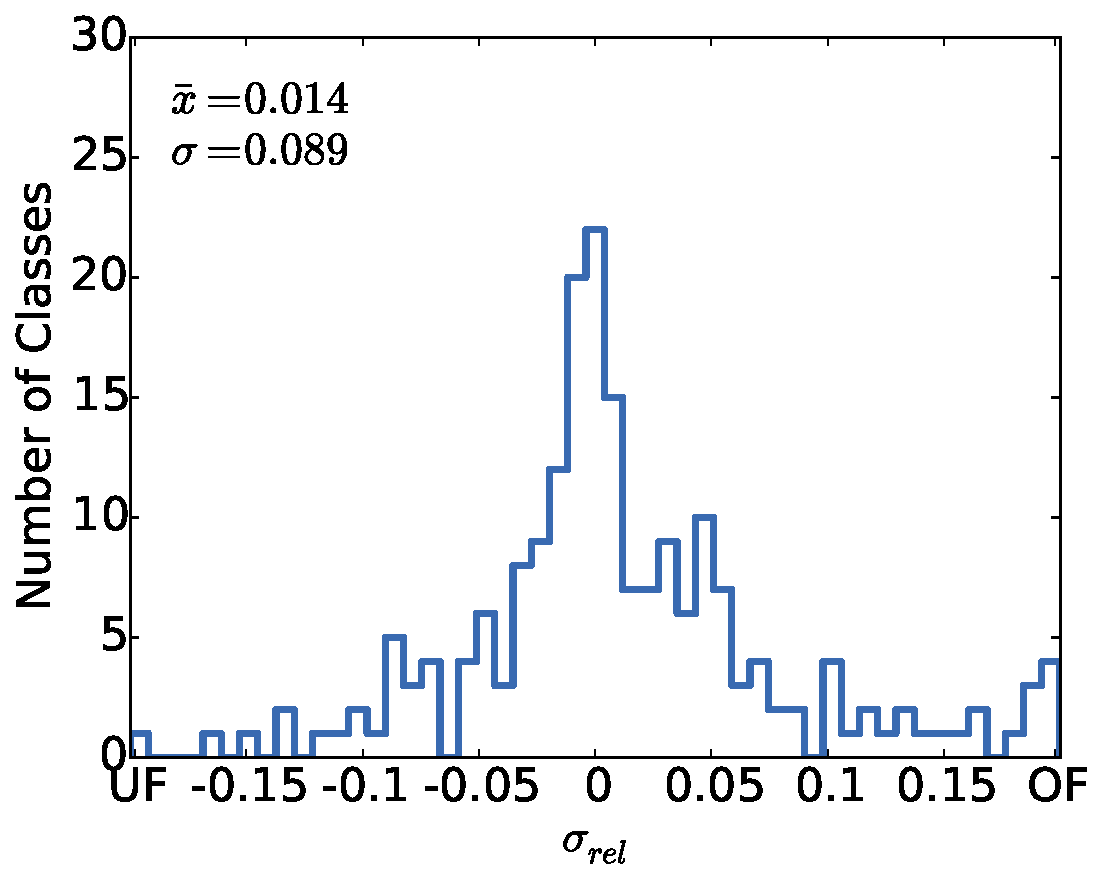
\includegraphics[width=0.49\textwidth]{delta_p_tilde_validation_f2vqs1} \\
	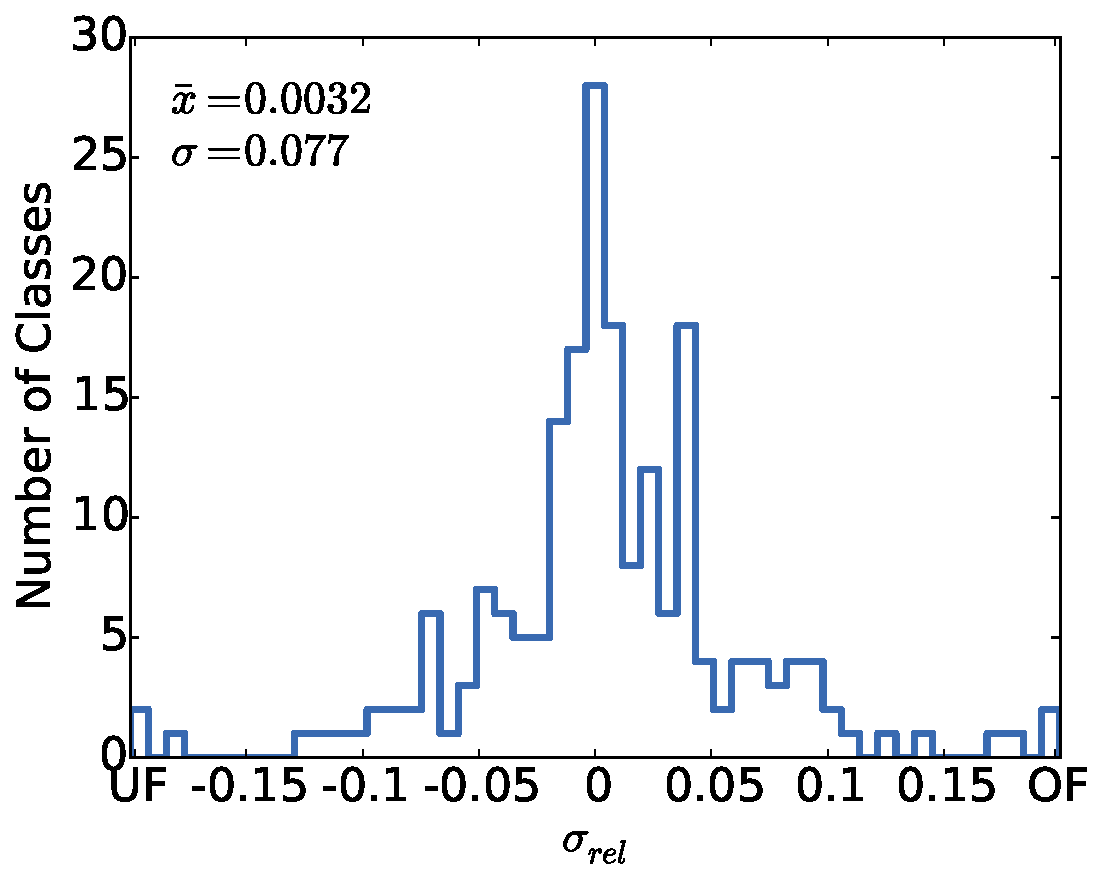
\includegraphics[width=0.49\textwidth]{delta_p_tilde_validation_f1vqs2}
	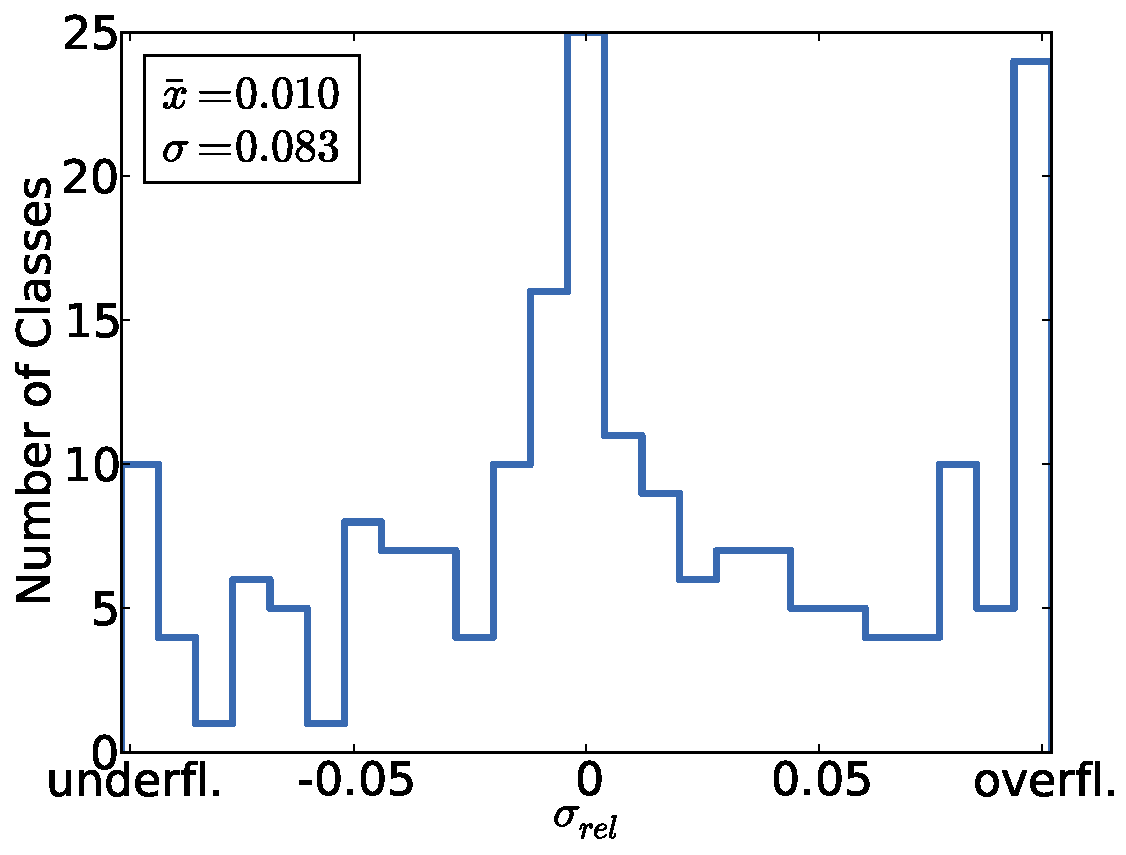
\includegraphics[width=0.49\textwidth]{delta_p_tilde_validation_f2vqs2} \\
	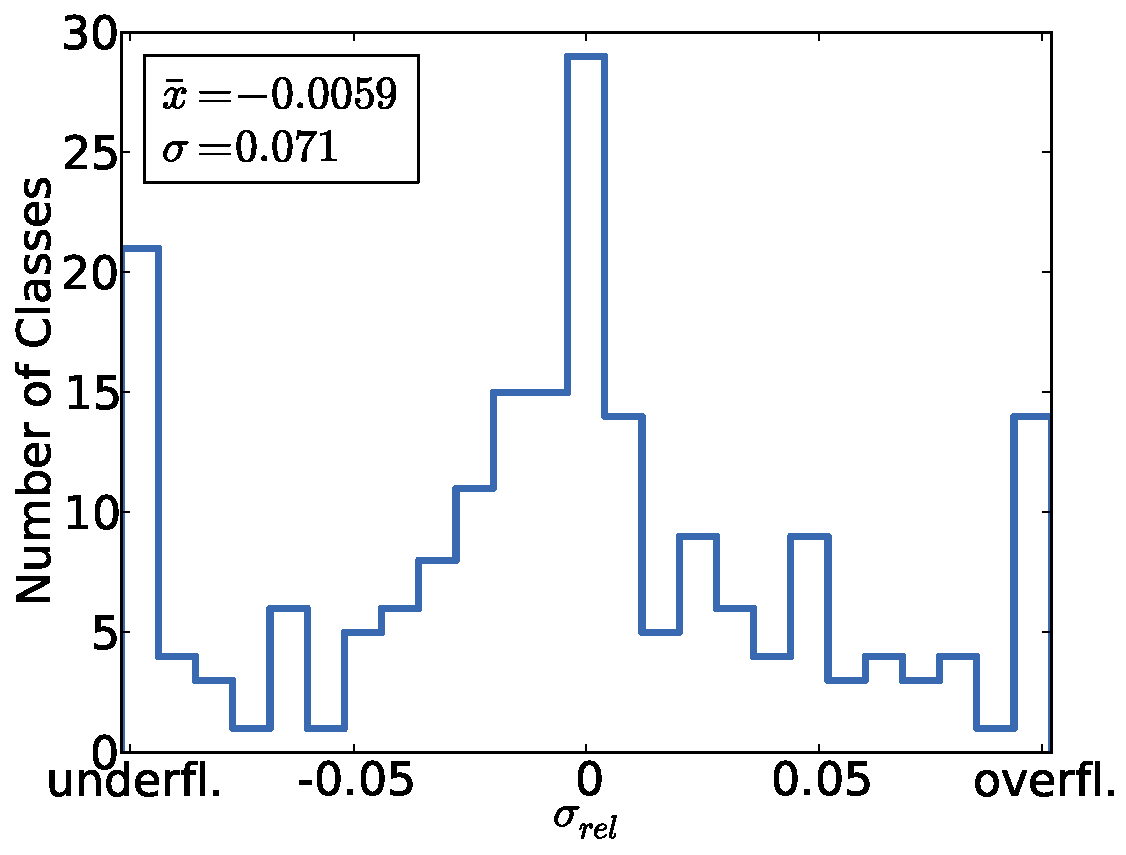
\includegraphics[width=0.49\textwidth]{delta_p_tilde_validation_f1vqs3}
	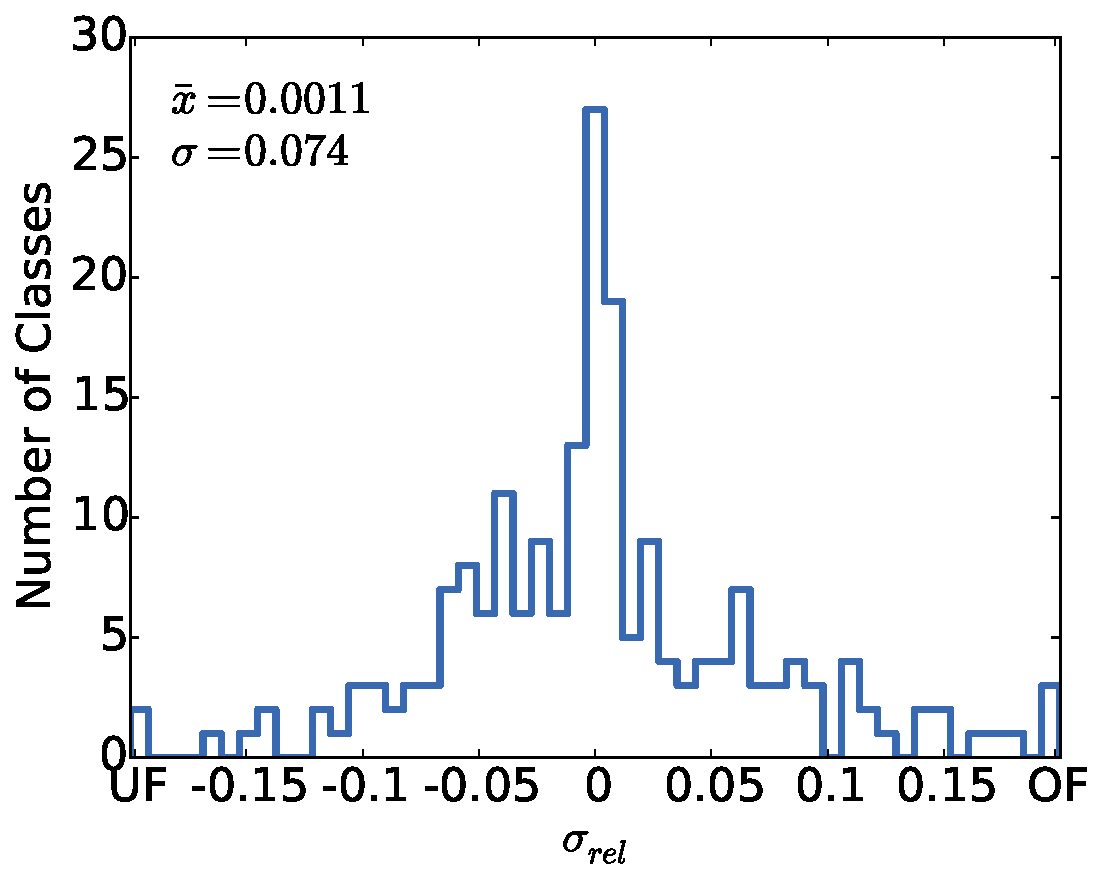
\includegraphics[width=0.49\textwidth]{delta_p_tilde_validation_f2vqs3} \\
	\caption{Distribution of the relative \ptilde deviation \sigmarel. \\Top: comparison between two full scan runs. \\Left side: comparison between full scan run \num{1} and the Quickscan runs \numrange{1}{3}. \\Right side: comparison between full scan run \num{2} and the Quickscan runs \numrange{1}{3}.}
	\label{fig:validation_result}
\end{figure}

The results of this validation run are illustrated in figure \ref{fig:validation_result}. The top figure shows the comparison between the two full scan runs. As expected, the  \sigmarel distribution shows a finite width due to random influences. The other six histograms show the comparison between the full scans and each of the three Quickscan results.
None of the distribution means is significantly shifted away from \num{0}. The distribution widths are within their deviations compatible with the broadening due to random fluctuations.

Since the number of pseudo-experiments is significantly greater in this scenario, the constant computation overhead has less influence on the computation time. As shown in table \ref{tbl:validation_speedup}, a speedup of \num{9.2 +- 0.5} times is achieved.

\begin{table}
	\centering
	\begin{tabular}{ l S[table-format=5] l l }
		\toprule
		\multicolumn{1}{c}{} & {Measurement / \si{\second}} & {Combined / \si{\second}} & {Speedup} \\ 
		\midrule
		Full Scan 1 & 28684 & \multirow{2}{*}{\tablenum[table-format=5(4)]{30373 +- 1689}} & \multirow{5}{*}{\num{9.2 +- 0.5}} \\
		Full Scan 2 & 32062 & & \\
		\cmidrule{1-2}
		Quickscan 1 & 3386 & \multirow{3}{*}{\tablenum[table-format=5(4)]{3310 +- 52}} & \\
		Quickscan 2 & 3212 & & \\
		Quickscan 3 & 3334 & & \\
		\bottomrule
	\end{tabular}
	\caption{Results for the computation time measurement in seconds. Two full scan trials and three Quickscan trials are performed. The second column shows the combined result as mean and its error.}
	\label{tbl:validation_speedup}
\end{table}

Overall, the validation run has shown that the parameter choice $ \paramregions = \num{200} $ is reasonable. With the aid of the Quickscan, the computation time could be decreased by a factor of about \num{9} without changing the results.